Since each leg has three degrees of freedom, there are three angles that need to be controlled in order to move the leg to a desired position. These will be referred to as theta ($\theta$), phi($\phi$) and alpha($\alpha$) throughout this document. Theta describes the horizontal angle between the tangent of the body and leg segment A as shown in Figure \ref{fig:Leg_design_2}. 

\FloatBarrier
\begin{figure}[h]
\centering
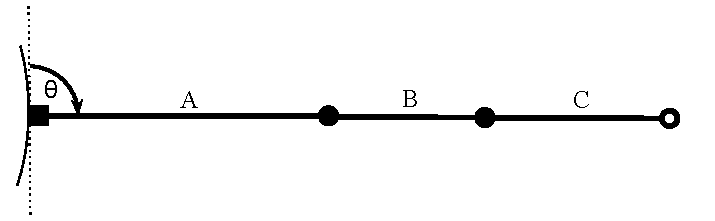
\includegraphics[scale = 1]{pics/Leg_design_2.pdf}
\caption{Top view of the leg design model for mathematical analysis.}
\label{fig:Leg_design_2}
\end{figure}
\FloatBarrier

Phi describes the angle between leg segments A and B viewed directly from the side. In the same plane, alpha describes the angle between leg segments B and C. Both of these angles can be seen in Figure \ref{fig:Leg_design}.

\FloatBarrier
\begin{figure}[h]
\centering
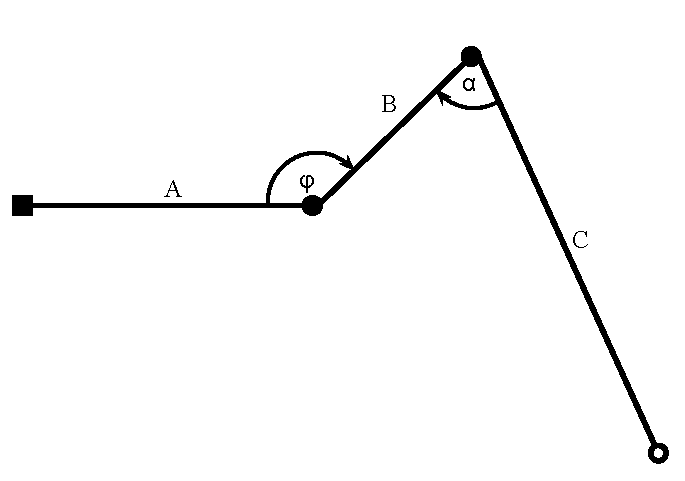
\includegraphics[scale = 1]{pics/Leg_design.pdf}
\caption{Side view of the leg design model for mathematical analysis.}
\label{fig:Leg_design}
\end{figure}
\FloatBarrier

In order to control the robot in a Cartesian world it is necessary to find a transfer function for a leg that can translate a coordinate vector in the domain $[\theta,\phi,\alpha]$ to a vector in the domain $[x,y,z]$. This is done through mathematical analysis of a single leg.\\

By using Figure \ref{fig:Leg_design_2} and some simple trigonometry, theta can be found to be

\begin{align}
\theta = arctan\Big(\frac{x}{y}\Big)
\end{align}

where \textit{x}, \textit{y} and \textit{z} are the desired coordinates for the foot of the relevant leg. It is important to note that the hip of the leg where section A meets the chassis is the origin of the Cartesian system for this analysis. This can be seen in Figure \ref{fig:Leg_design_3}

\FloatBarrier
\begin{figure}[h]
\centering
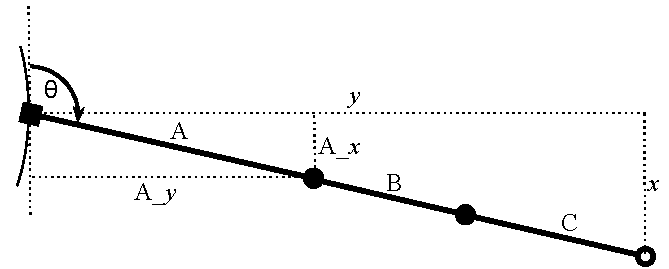
\includegraphics[scale = 1]{pics/Leg_design_3.pdf}
\caption{Annotated top view of the leg design model for mathematical analysis.}
\label{fig:Leg_design_3}
\end{figure}
\FloatBarrier

In order to do an analysis on phi and alpha, it is necessary to add a few construction lines to the generic model in Figure \ref{fig:Leg_design}. The additions can be seen in Figure \ref{fig:Leg_design_4} and the additions are explained below.

\begin{figure}[h]
\centering
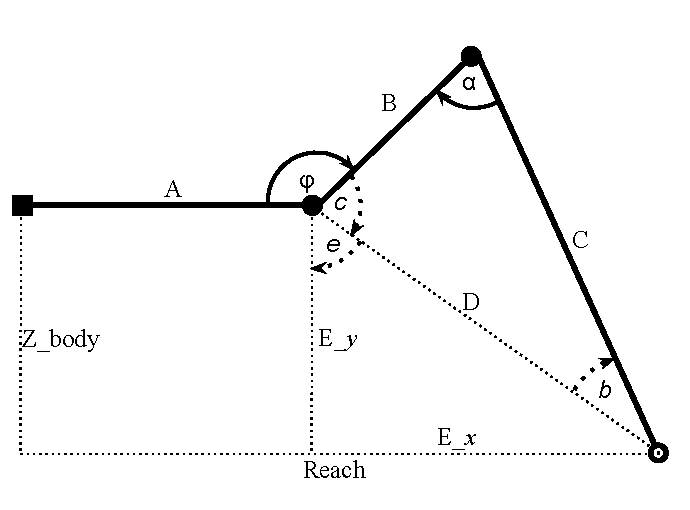
\includegraphics[scale = 1]{pics/Leg_design_4.pdf}
\caption{Annotated side view of the leg design model for mathematical analysis.}
\label{fig:Leg_design_4}
\end{figure}

From Figure 8:
\begin{itemize}
\item $Z_{body}$ is the nominal height difference between the robot chassis and ground. This value is a constant.
\item \textit{Reach} is the horizontal distance between the hip and the foot.
\item \textit{D} is an imaginary line between joint 2 and the foot that completes the triangle \textit{BCD} that will form the basis of this analysis.
\item $E_x$ is the horizontal distance between joint 2 and the foot.
\item $E_y$ is the horizontal line that completes triangle $DE_xE_y$. Quantitatively $E_y = Z_{body}$ since the ground is assumed to be level in this analysis.
\item \textit{c} is the angle between $B$ and $D$.
\item \textit{b} is the angle between $C$ and $D$.
\item \textit{e} is the angle between $E_y$ and $D$.
\end{itemize}

\begin{align}
\therefore Reach = \sqrt{x^2+y^2}
\end{align}

By using triangle \textit{BCD} and the Cosine rule,

\begin{align}
cos(\alpha) &= \frac{B^2+C^2-D^2}{2\times B\times C}\\
\therefore \alpha &= cos^{-1}\Bigg(\frac{B^2+C^2-D^2}{2\times B\times C}\Bigg).
\end{align}

The value of $E_x$ can be calculated similar to that of reach, but first finding the $x$ and $y$ component lengths of segment A as shown in Figure \ref{fig:Leg_design_3}.

\begin{align}
A_x &= A \times sin(\theta)\\
A_y &= A \times cos(\theta)\\
E_x &= \sqrt{(x-A_x)^2+(y-A_y)^2}
\end{align}
The Sine rule can then be used on triangle $DE_xE_y$ to find,

\begin{align}
\frac{sin(c)}{C} &= \frac{sin(\alpha)}{D}\\
\therefore sin(c) &= C \times \frac{sin(\alpha)}{D}\\
\therefore c &= sin^{-1}\Bigg(C \times \frac{sin(\alpha)}{D}\Bigg).
\end{align}

Angle \textit{e} can easily be found as

\begin{align}
e = tan^{-1}\Bigg(\frac{E_x}{E_y}\Bigg).
\end{align}

With all of this calculated, phi can be calculated as

\begin{align}
\phi = 270^o - c -e.
\end{align}

The analysis above is valid for the generic 3 segment design shown in Figures \ref{fig:Leg_design_2} and \ref{fig:Leg_design} where the hip is at the origin of the Cartesian system. The real robot has five legs that need to be calculated for. In order to avoid using five different Cartesian systems, it is necessary to be able to rotate and translate this generic model to suit the requirements of any of the legs.\\

\FloatBarrier
\begin{figure}[h]
\centering
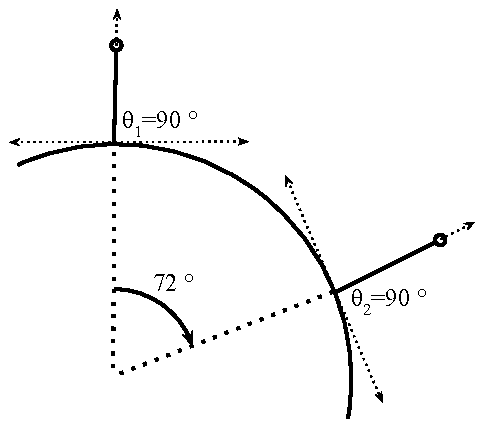
\includegraphics[scale = 1]{pics/Body_Layout_2.pdf}
\caption{Top view of the robot showing individual Cartesian systems for individual legs.}
\label{fig:Body_layout_2}
\end{figure}
\FloatBarrier

Figure \ref{fig:Body_layout_2} illustrates that both leg 1 and 2 have a theta angle of $\theta = 90^o$, yet they are clearly not facing the same direction. This is because of this separate coordinate system that each of the legs have in order to do the inverse kinematic calculations. In order to do calculations on the whole robot, the centre of the robot is used as the origin.\\

If \textit{leg} denotes the number of the desired leg, a leg's coordinate system can be rotated by using

\begin{align}
(x',y') &= (x\times cos(\gamma) -y\times sin(\gamma),x \times sin(\gamma) + y \times cos(\gamma))\\
\text{where }\gamma &= (leg-1)\times 72^o. 
\end{align}

For the robot to be able to walk, all five legs should be working together to move in a specific direction. The use of vectors work well since they can be added easily and contain both direction and magnitude information. The movement of each foot can be constrained for each of the bends $(\theta,\phi,\alpha)$ to limit the angle to a realistic value for the servo. These limitations can be seen in Figure \ref{fig:Body_layout_3} as dotted lines. The dashed line represents the vector for movement. The movement vector is limited by the boundary.

\FloatBarrier
\begin{figure}[h]
\centering
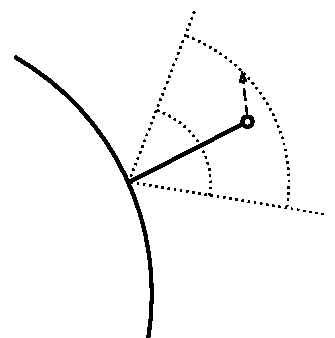
\includegraphics[scale = 1]{pics/Body_Layout_3.pdf}
\caption{Top view of the robot showing the addition of vectors and leg boundaries.}
\label{fig:Body_layout_3}
\end{figure}
\FloatBarrier

All of the legs move together towards a point inside or on the edge of each individual perimeter. The direction of movement of the robot can be calculated as

\begin{align}
angle = arctan \Bigg(\frac{y}{x}\Bigg),
\end{align}
where $x$ and $y$ denote the input from the user interface. The magnitude can be found to be
\begin{align}
magnitude = \sqrt{x^2+y^2}.
\end{align}
The magnitude and direction can be used to check if the vector fits inside the perimeter.\\

All of the calculations above only account for translation, that is moving forward, backward, left, right or a combination of the above. Being able to move truly holonomically means being able to rotate with or without translating. The vectors used to calculate the trajectory of each leg works well for representing translation but does not work so well for rotation. Rotation can instead be expressed as a scalar value, which has magnitude and a sign indicating the direction of rotation. A positive value indicates a clockwise rotation. When these rotation vectors are applied to the individual legs, it results in a different vector being added to each leg indicating the trajectory required by each leg to rotate the robot body. Figure \ref{fig:Body_layout_4} shows the effect of adding a rotation scalar to the movement. The dashed arrows indicate the trajectory of each individual leg.

\FloatBarrier
\begin{figure}[h]
\centering
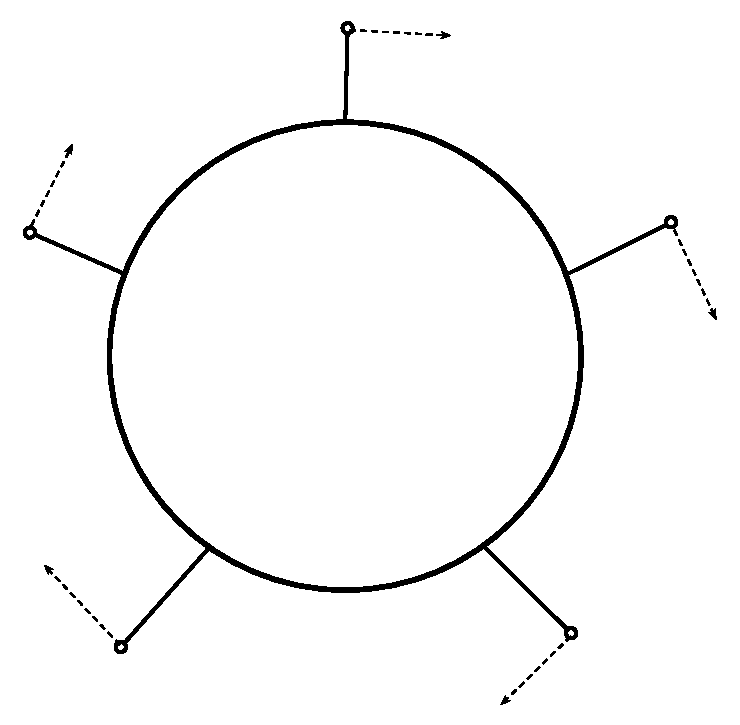
\includegraphics[scale = 1]{pics/Body_Layout_4.pdf}
\caption{Top view of the robot showing the addition of vectors for rotation about the origin.}
\label{fig:Body_layout_4}
\end{figure}
\FloatBarrier

If each leg were instructed to follow the dashed arrows shown in Figure \ref{fig:Body_layout_4}, the legs would fight each other for grip since they vectors will force them to spread out. Since this is not a controlled movement. Simply using the instantaneous trajectory as the movement vector will not work like it did in the case of translational movement. Instead the trajectory will constantly be changing to keep rotate the body while keeping the feet in their positions. This change can be seen in Figure 